\documentclass[1p]{elsarticle_modified}
%\bibliographystyle{elsarticle-num}

%\usepackage[colorlinks]{hyperref}
%\usepackage{abbrmath_seonhwa} %\Abb, \Ascr, \Acal ,\Abf, \Afrak
\usepackage{amsfonts}
\usepackage{amssymb}
\usepackage{amsmath}
\usepackage{amsthm}
\usepackage{scalefnt}
\usepackage{amsbsy}
\usepackage{kotex}
\usepackage{caption}
\usepackage{subfig}
\usepackage{color}
\usepackage{graphicx}
\usepackage{xcolor} %% white, black, red, green, blue, cyan, magenta, yellow
\usepackage{float}
\usepackage{setspace}
\usepackage{hyperref}

\usepackage{tikz}
\usetikzlibrary{arrows}

\usepackage{multirow}
\usepackage{array} % fixed length table
\usepackage{hhline}

%%%%%%%%%%%%%%%%%%%%%
\makeatletter
\renewcommand*\env@matrix[1][\arraystretch]{%
	\edef\arraystretch{#1}%
	\hskip -\arraycolsep
	\let\@ifnextchar\new@ifnextchar
	\array{*\c@MaxMatrixCols c}}
\makeatother %https://tex.stackexchange.com/questions/14071/how-can-i-increase-the-line-spacing-in-a-matrix
%%%%%%%%%%%%%%%

\usepackage[normalem]{ulem}

\newcommand{\msout}[1]{\ifmmode\text{\sout{\ensuremath{#1}}}\else\sout{#1}\fi}
%SOURCE: \msout is \stkout macro in https://tex.stackexchange.com/questions/20609/strikeout-in-math-mode

\newcommand{\cancel}[1]{
	\ifmmode
	{\color{red}\msout{#1}}
	\else
	{\color{red}\sout{#1}}
	\fi
}

\newcommand{\add}[1]{
	{\color{blue}\uwave{#1}}
}

\newcommand{\replace}[2]{
	\ifmmode
	{\color{red}\msout{#1}}{\color{blue}\uwave{#2}}
	\else
	{\color{red}\sout{#1}}{\color{blue}\uwave{#2}}
	\fi
}

\newcommand{\Sol}{\mathcal{S}} %segment
\newcommand{\D}{D} %diagram
\newcommand{\A}{\mathcal{A}} %arc


%%%%%%%%%%%%%%%%%%%%%%%%%%%%%5 test

\def\sl{\operatorname{\textup{SL}}(2,\Cbb)}
\def\psl{\operatorname{\textup{PSL}}(2,\Cbb)}
\def\quan{\mkern 1mu \triangleright \mkern 1mu}

\theoremstyle{definition}
\newtheorem{thm}{Theorem}[section]
\newtheorem{prop}[thm]{Proposition}
\newtheorem{lem}[thm]{Lemma}
\newtheorem{ques}[thm]{Question}
\newtheorem{cor}[thm]{Corollary}
\newtheorem{defn}[thm]{Definition}
\newtheorem{exam}[thm]{Example}
\newtheorem{rmk}[thm]{Remark}
\newtheorem{alg}[thm]{Algorithm}

\newcommand{\I}{\sqrt{-1}}
\begin{document}

%\begin{frontmatter}
%
%\title{Boundary parabolic representations of knots up to 8 crossings}
%
%%% Group authors per affiliation:
%\author{Yunhi Cho} 
%\address{Department of Mathematics, University of Seoul, Seoul, Korea}
%\ead{yhcho@uos.ac.kr}
%
%
%\author{Seonhwa Kim} %\fnref{s_kim}}
%\address{Center for Geometry and Physics, Institute for Basic Science, Pohang, 37673, Korea}
%\ead{ryeona17@ibs.re.kr}
%
%\author{Hyuk Kim}
%\address{Department of Mathematical Sciences, Seoul National University, Seoul 08826, Korea}
%\ead{hyukkim@snu.ac.kr}
%
%\author{Seokbeom Yoon}
%\address{Department of Mathematical Sciences, Seoul National University, Seoul, 08826,  Korea}
%\ead{sbyoon15@snu.ac.kr}
%
%\begin{abstract}
%We find all boundary parabolic representation of knots up to 8 crossings.
%
%\end{abstract}
%\begin{keyword}
%    \MSC[2010] 57M25 
%\end{keyword}
%
%\end{frontmatter}

%\linenumbers
%\tableofcontents
%
\newcommand\colored[1]{\textcolor{white}{\rule[-0.35ex]{0.8em}{1.4ex}}\kern-0.8em\color{red} #1}%
%\newcommand\colored[1]{\textcolor{white}{ #1}\kern-2.17ex	\textcolor{white}{ #1}\kern-1.81ex	\textcolor{white}{ #1}\kern-2.15ex\color{red}#1	}

{\Large $\underline{12n_{0360}~(K12n_{0360})}$}

\setlength{\tabcolsep}{10pt}
\renewcommand{\arraystretch}{1.6}
\vspace{1cm}\begin{tabular}{m{100pt}>{\centering\arraybackslash}m{274pt}}
\multirow{5}{120pt}{
	\centering
	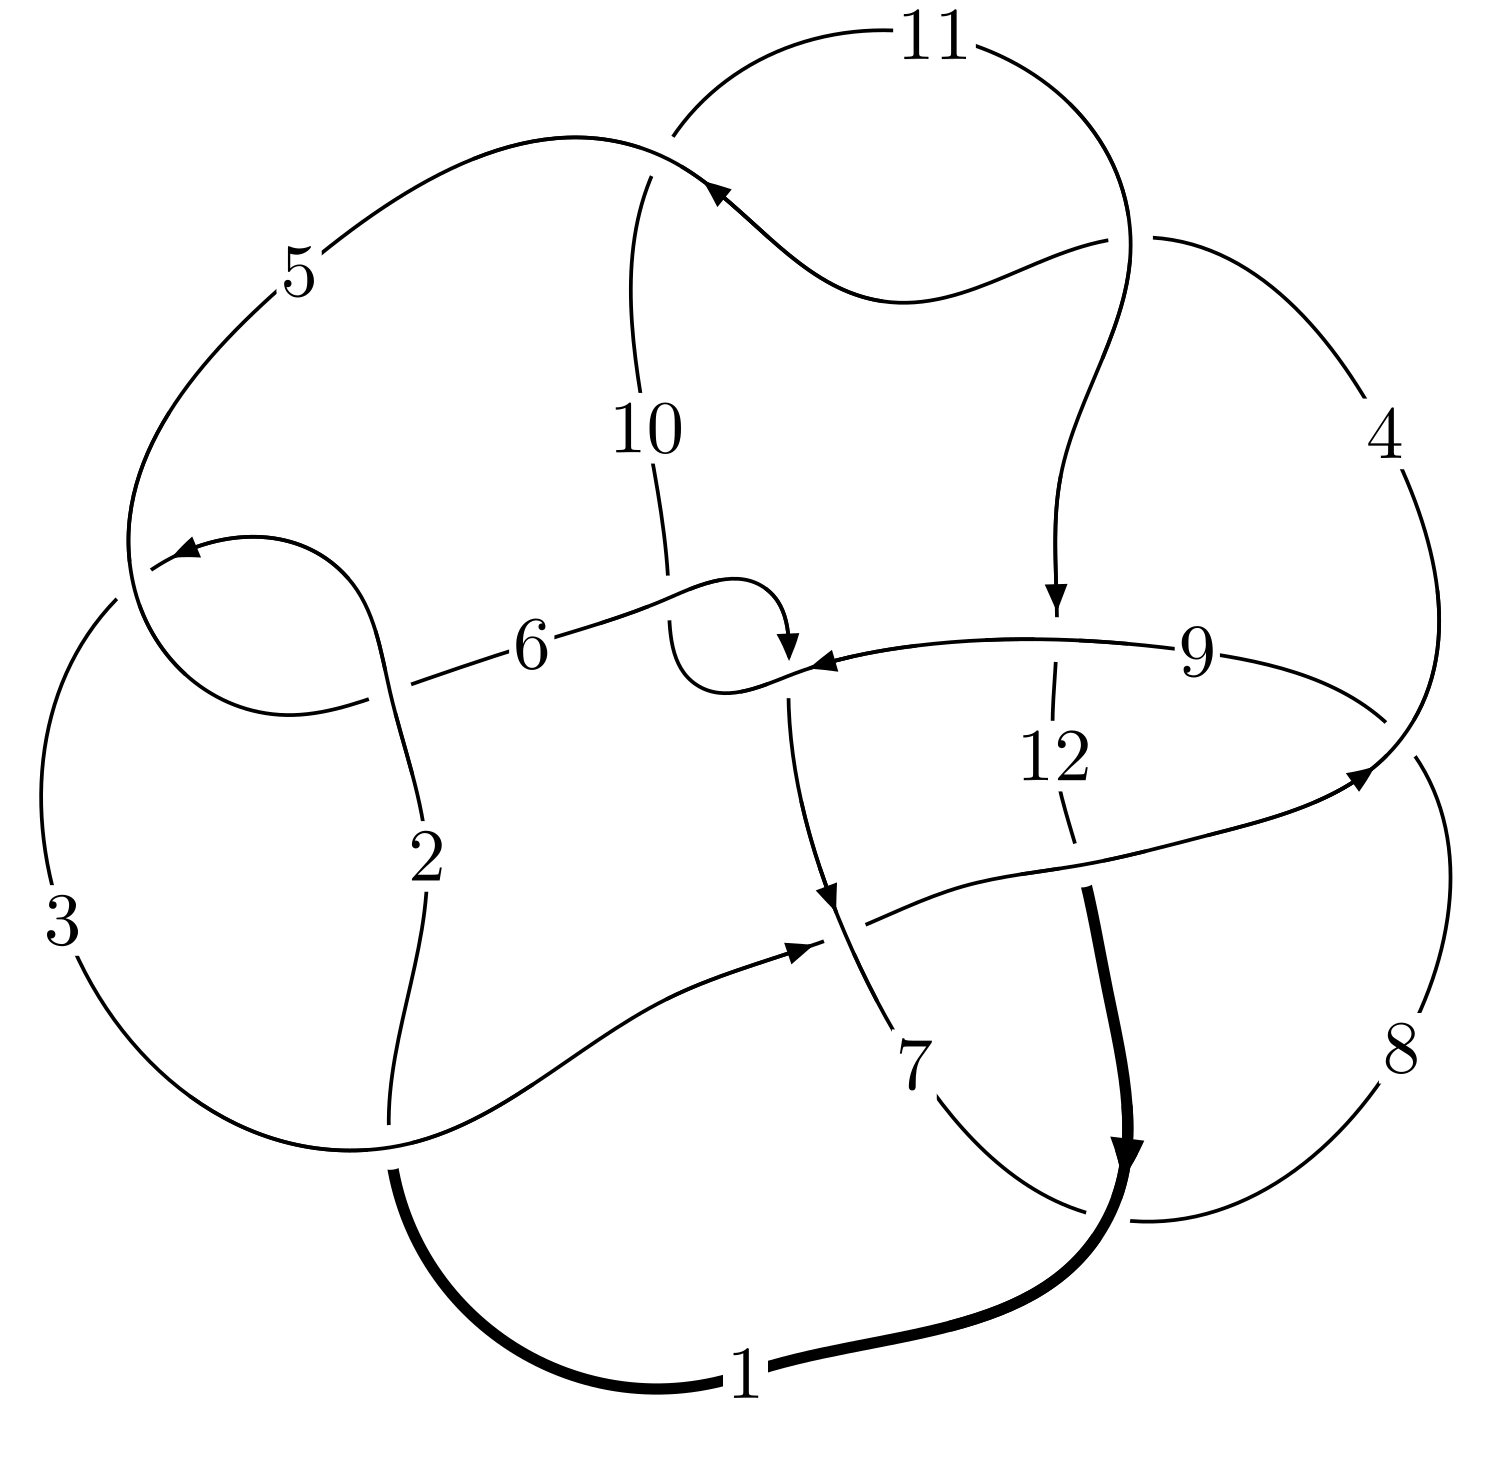
\includegraphics[width=112pt]{../../../GIT/diagram.site/Diagrams/png/2449_12n_0360.png}\\
\ \ \ A knot diagram\footnotemark}&
\allowdisplaybreaks
\textbf{Linearized knot diagam} \\
\cline{2-2}
 &
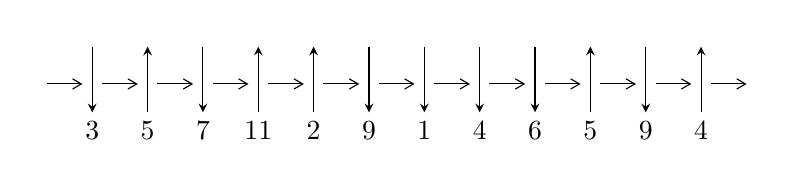
\begin{tikzpicture}[x=20pt, y=17pt]
	% nodes
	\node (C0) at (0, 0) {};
	\node (C1) at (1, 0) {};
	\node (C1U) at (1, +1) {};
	\node (C1D) at (1, -1) {3};

	\node (C2) at (2, 0) {};
	\node (C2U) at (2, +1) {};
	\node (C2D) at (2, -1) {5};

	\node (C3) at (3, 0) {};
	\node (C3U) at (3, +1) {};
	\node (C3D) at (3, -1) {7};

	\node (C4) at (4, 0) {};
	\node (C4U) at (4, +1) {};
	\node (C4D) at (4, -1) {11};

	\node (C5) at (5, 0) {};
	\node (C5U) at (5, +1) {};
	\node (C5D) at (5, -1) {2};

	\node (C6) at (6, 0) {};
	\node (C6U) at (6, +1) {};
	\node (C6D) at (6, -1) {9};

	\node (C7) at (7, 0) {};
	\node (C7U) at (7, +1) {};
	\node (C7D) at (7, -1) {1};

	\node (C8) at (8, 0) {};
	\node (C8U) at (8, +1) {};
	\node (C8D) at (8, -1) {4};

	\node (C9) at (9, 0) {};
	\node (C9U) at (9, +1) {};
	\node (C9D) at (9, -1) {6};

	\node (C10) at (10, 0) {};
	\node (C10U) at (10, +1) {};
	\node (C10D) at (10, -1) {5};

	\node (C11) at (11, 0) {};
	\node (C11U) at (11, +1) {};
	\node (C11D) at (11, -1) {9};

	\node (C12) at (12, 0) {};
	\node (C12U) at (12, +1) {};
	\node (C12D) at (12, -1) {4};
	\node (C13) at (13, 0) {};

	% arrows
	\draw[->,>={angle 60}]
	(C0) edge (C1) (C1) edge (C2) (C2) edge (C3) (C3) edge (C4) (C4) edge (C5) (C5) edge (C6) (C6) edge (C7) (C7) edge (C8) (C8) edge (C9) (C9) edge (C10) (C10) edge (C11) (C11) edge (C12) (C12) edge (C13) ;	\draw[->,>=stealth]
	(C1U) edge (C1D) (C2D) edge (C2U) (C3U) edge (C3D) (C4D) edge (C4U) (C5D) edge (C5U) (C6U) edge (C6D) (C7U) edge (C7D) (C8U) edge (C8D) (C9U) edge (C9D) (C10D) edge (C10U) (C11U) edge (C11D) (C12D) edge (C12U) ;
	\end{tikzpicture} \\
\hhline{~~} \\& 
\textbf{Solving Sequence} \\ \cline{2-2} 
 &
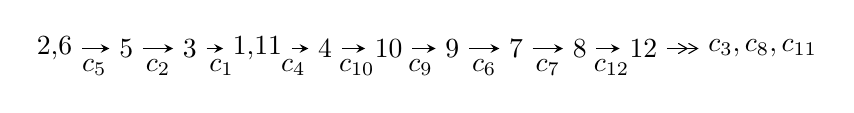
\begin{tikzpicture}[x=23pt, y=7pt]
	% node
	\node (A0) at (-1/8, 0) {2,6};
	\node (A1) at (1, 0) {5};
	\node (A2) at (2, 0) {3};
	\node (A3) at (49/16, 0) {1,11};
	\node (A4) at (33/8, 0) {4};
	\node (A5) at (41/8, 0) {10};
	\node (A6) at (49/8, 0) {9};
	\node (A7) at (57/8, 0) {7};
	\node (A8) at (65/8, 0) {8};
	\node (A9) at (73/8, 0) {12};
	\node (C1) at (1/2, -1) {$c_{5}$};
	\node (C2) at (3/2, -1) {$c_{2}$};
	\node (C3) at (5/2, -1) {$c_{1}$};
	\node (C4) at (29/8, -1) {$c_{4}$};
	\node (C5) at (37/8, -1) {$c_{10}$};
	\node (C6) at (45/8, -1) {$c_{9}$};
	\node (C7) at (53/8, -1) {$c_{6}$};
	\node (C8) at (61/8, -1) {$c_{7}$};
	\node (C9) at (69/8, -1) {$c_{12}$};
	\node (A10) at (11, 0) {$c_{3},c_{8},c_{11}$};

	% edge
	\draw[->,>=stealth]	
	(A0) edge (A1) (A1) edge (A2) (A2) edge (A3) (A3) edge (A4) (A4) edge (A5) (A5) edge (A6) (A6) edge (A7) (A7) edge (A8) (A8) edge (A9) ;
	\draw[->>,>={angle 60}]	
	(A9) edge (A10);
\end{tikzpicture} \\ 

\end{tabular} \\

\footnotetext{
The image of knot diagram is generated by the software ``\textbf{Draw programme}" developed by Andrew Bartholomew(\url{http://www.layer8.co.uk/maths/draw/index.htm\#Running-draw}), where we modified some parts for our purpose(\url{https://github.com/CATsTAILs/LinksPainter}).
}\phantom \\ \newline 
\centering \textbf{Ideals for irreducible components\footnotemark of $X_{\text{par}}$} 
 
\begin{align*}
I^u_{1}&=\langle 
-3.17231\times10^{41} u^{41}-1.10310\times10^{41} u^{40}+\cdots+1.27534\times10^{41} b-1.91700\times10^{42},\\
\phantom{I^u_{1}}&\phantom{= \langle  }-3.79921\times10^{42} u^{41}+1.16103\times10^{42} u^{40}+\cdots+1.27534\times10^{41} a-5.15011\times10^{42},\;u^{42}+4 u^{40}+\cdots+8 u+1\rangle \\
I^u_{2}&=\langle 
-4867 u^{17}+14254 u^{16}+\cdots+1012 b+2283,\;-6343 u^{17}+8982 u^{16}+\cdots+1012 a-18113,\\
\phantom{I^u_{2}}&\phantom{= \langle  }u^{18}-3 u^{17}+\cdots-2 u+1\rangle \\
\\
\end{align*}
\raggedright * 2 irreducible components of $\dim_{\mathbb{C}}=0$, with total 60 representations.\\
\footnotetext{All coefficients of polynomials are rational numbers. But the coefficients are sometimes approximated in decimal forms when there is not enough margin.}
\newpage
\renewcommand{\arraystretch}{1}
\centering \section*{I. $I^u_{1}= \langle -3.17\times10^{41} u^{41}-1.10\times10^{41} u^{40}+\cdots+1.28\times10^{41} b-1.92\times10^{42},\;-3.80\times10^{42} u^{41}+1.16\times10^{42} u^{40}+\cdots+1.28\times10^{41} a-5.15\times10^{42},\;u^{42}+4 u^{40}+\cdots+8 u+1 \rangle$}
\flushleft \textbf{(i) Arc colorings}\\
\begin{tabular}{m{7pt} m{180pt} m{7pt} m{180pt} }
\flushright $a_{2}=$&$\begin{pmatrix}0\\u\end{pmatrix}$ \\
\flushright $a_{6}=$&$\begin{pmatrix}1\\0\end{pmatrix}$ \\
\flushright $a_{5}=$&$\begin{pmatrix}1\\u^2\end{pmatrix}$ \\
\flushright $a_{3}=$&$\begin{pmatrix}u\\u^3+u\end{pmatrix}$ \\
\flushright $a_{1}=$&$\begin{pmatrix}u^3\\u^5+u^3+u\end{pmatrix}$ \\
\flushright $a_{11}=$&$\begin{pmatrix}29.7898 u^{41}-9.10368 u^{40}+\cdots+352.163 u+40.3823\\2.48742 u^{41}+0.864947 u^{40}+\cdots+84.3991 u+15.0313\end{pmatrix}$ \\
\flushright $a_{4}=$&$\begin{pmatrix}-18.2967 u^{41}-1.79519 u^{40}+\cdots-427.707 u-64.5574\\1.07748 u^{41}+0.260227 u^{40}+\cdots+14.9654 u-0.377505\end{pmatrix}$ \\
\flushright $a_{10}=$&$\begin{pmatrix}26.3588 u^{41}-7.38711 u^{40}+\cdots+310.803 u+34.4547\\2.06799 u^{41}+0.593466 u^{40}+\cdots+74.0976 u+13.3147\end{pmatrix}$ \\
\flushright $a_{9}=$&$\begin{pmatrix}28.4268 u^{41}-6.79364 u^{40}+\cdots+384.901 u+47.7694\\2.06799 u^{41}+0.593466 u^{40}+\cdots+74.0976 u+13.3147\end{pmatrix}$ \\
\flushright $a_{7}=$&$\begin{pmatrix}8.01480 u^{41}-7.35645 u^{40}+\cdots-49.3603 u-18.0733\\5.08682 u^{41}+0.163226 u^{40}+\cdots+86.5337 u+9.31672\end{pmatrix}$ \\
\flushright $a_{8}=$&$\begin{pmatrix}7.63267 u^{41}-7.14139 u^{40}+\cdots-53.0896 u-18.3070\\6.44055 u^{41}+0.639959 u^{40}+\cdots+130.209 u+16.3404\end{pmatrix}$ \\
\flushright $a_{12}=$&$\begin{pmatrix}19.0918 u^{41}+7.25817 u^{40}+\cdots+568.854 u+93.4086\\-1.69590 u^{41}+4.74779 u^{40}+\cdots+94.9034 u+19.8886\end{pmatrix}$\\&\end{tabular}
\flushleft \textbf{(ii) Obstruction class $= -1$}\\~\\
\flushleft \textbf{(iii) Cusp Shapes $= 29.4758 u^{41}-5.89551 u^{40}+\cdots+439.594 u+56.8690$}\\~\\
\newpage\renewcommand{\arraystretch}{1}
\flushleft \textbf{(iv) u-Polynomials at the component}\newline \\
\begin{tabular}{m{50pt}|m{274pt}}
Crossings & \hspace{64pt}u-Polynomials at each crossing \\
\hline $$\begin{aligned}c_{1}\end{aligned}$$&$\begin{aligned}
&u^{42}+8 u^{41}+\cdots+14 u+1
\end{aligned}$\\
\hline $$\begin{aligned}c_{2},c_{5}\end{aligned}$$&$\begin{aligned}
&u^{42}+4 u^{40}+\cdots+8 u+1
\end{aligned}$\\
\hline $$\begin{aligned}c_{3}\end{aligned}$$&$\begin{aligned}
&u^{42}+u^{41}+\cdots+15 u+1
\end{aligned}$\\
\hline $$\begin{aligned}c_{4},c_{10}\end{aligned}$$&$\begin{aligned}
&u^{42}-3 u^{40}+\cdots+3884 u+653
\end{aligned}$\\
\hline $$\begin{aligned}c_{6},c_{9}\end{aligned}$$&$\begin{aligned}
&u^{42}-2 u^{41}+\cdots-1450 u+2881
\end{aligned}$\\
\hline $$\begin{aligned}c_{7},c_{11}\end{aligned}$$&$\begin{aligned}
&u^{42}-2 u^{41}+\cdots+102 u+116
\end{aligned}$\\
\hline $$\begin{aligned}c_{8}\end{aligned}$$&$\begin{aligned}
&u^{42}+29 u^{40}+\cdots-3172 u+968
\end{aligned}$\\
\hline $$\begin{aligned}c_{12}\end{aligned}$$&$\begin{aligned}
&u^{42}+u^{41}+\cdots+8821 u+713
\end{aligned}$\\
\hline
\end{tabular}\\~\\
\newpage\renewcommand{\arraystretch}{1}
\flushleft \textbf{(v) Riley Polynomials at the component}\newline \\
\begin{tabular}{m{50pt}|m{274pt}}
Crossings & \hspace{64pt}Riley Polynomials at each crossing \\
\hline $$\begin{aligned}c_{1}\end{aligned}$$&$\begin{aligned}
&y^{42}+60 y^{41}+\cdots+106 y+1
\end{aligned}$\\
\hline $$\begin{aligned}c_{2},c_{5}\end{aligned}$$&$\begin{aligned}
&y^{42}+8 y^{41}+\cdots+14 y+1
\end{aligned}$\\
\hline $$\begin{aligned}c_{3}\end{aligned}$$&$\begin{aligned}
&y^{42}+7 y^{41}+\cdots+461 y+1
\end{aligned}$\\
\hline $$\begin{aligned}c_{4},c_{10}\end{aligned}$$&$\begin{aligned}
&y^{42}-6 y^{41}+\cdots-6058384 y+426409
\end{aligned}$\\
\hline $$\begin{aligned}c_{6},c_{9}\end{aligned}$$&$\begin{aligned}
&y^{42}+54 y^{41}+\cdots+123416908 y+8300161
\end{aligned}$\\
\hline $$\begin{aligned}c_{7},c_{11}\end{aligned}$$&$\begin{aligned}
&y^{42}+50 y^{41}+\cdots+280292 y+13456
\end{aligned}$\\
\hline $$\begin{aligned}c_{8}\end{aligned}$$&$\begin{aligned}
&y^{42}+58 y^{41}+\cdots-12741008 y+937024
\end{aligned}$\\
\hline $$\begin{aligned}c_{12}\end{aligned}$$&$\begin{aligned}
&y^{42}-59 y^{41}+\cdots-9108213 y+508369
\end{aligned}$\\
\hline
\end{tabular}\\~\\
\newpage\flushleft \textbf{(vi) Complex Volumes and Cusp Shapes}
$$\begin{array}{c|c|c}  
\text{Solutions to }I^u_{1}& \I (\text{vol} + \sqrt{-1}CS) & \text{Cusp shape}\\
 \hline 
\begin{aligned}
u &= -0.401386 + 0.907950 I \\
a &= -1.30994 + 2.33702 I \\
b &= \phantom{-}1.61047 - 0.43509 I\end{aligned}
 & \phantom{-}5.91077 + 1.27313 I & \phantom{-}0.461828 + 0.968619 I \\ \hline\begin{aligned}
u &= -0.401386 - 0.907950 I \\
a &= -1.30994 - 2.33702 I \\
b &= \phantom{-}1.61047 + 0.43509 I\end{aligned}
 & \phantom{-}5.91077 - 1.27313 I & \phantom{-}0.461828 - 0.968619 I \\ \hline\begin{aligned}
u &= -0.482655 + 0.905869 I \\
a &= \phantom{-}1.53119 + 1.57511 I \\
b &= \phantom{-}0.357628 - 1.155570 I\end{aligned}
 & -3.09049 - 4.22260 I & -5.14689 + 7.39649 I \\ \hline\begin{aligned}
u &= -0.482655 - 0.905869 I \\
a &= \phantom{-}1.53119 - 1.57511 I \\
b &= \phantom{-}0.357628 + 1.155570 I\end{aligned}
 & -3.09049 + 4.22260 I & -5.14689 - 7.39649 I \\ \hline\begin{aligned}
u &= -0.703951 + 0.646413 I \\
a &= \phantom{-}0.097005 - 0.274142 I \\
b &= \phantom{-}1.35281 - 0.45723 I\end{aligned}
 & \phantom{-}7.00024 - 5.59064 I & \phantom{-}1.86038 + 6.99102 I \\ \hline\begin{aligned}
u &= -0.703951 - 0.646413 I \\
a &= \phantom{-}0.097005 + 0.274142 I \\
b &= \phantom{-}1.35281 + 0.45723 I\end{aligned}
 & \phantom{-}7.00024 + 5.59064 I & \phantom{-}1.86038 - 6.99102 I \\ \hline\begin{aligned}
u &= \phantom{-}0.284092 + 1.017050 I \\
a &= -0.211153 - 0.796137 I \\
b &= \phantom{-}0.270228 + 0.532970 I\end{aligned}
 & -0.93324 + 2.30287 I & \phantom{-}0.55695 - 5.43151 I \\ \hline\begin{aligned}
u &= \phantom{-}0.284092 - 1.017050 I \\
a &= -0.211153 + 0.796137 I \\
b &= \phantom{-}0.270228 - 0.532970 I\end{aligned}
 & -0.93324 - 2.30287 I & \phantom{-}0.55695 + 5.43151 I \\ \hline\begin{aligned}
u &= -0.344707 + 1.010570 I \\
a &= -0.70988 - 2.54288 I \\
b &= -1.04250 + 1.60858 I\end{aligned}
 & -3.88818 - 1.43090 I & -6.13404 - 0.44141 I \\ \hline\begin{aligned}
u &= -0.344707 - 1.010570 I \\
a &= -0.70988 + 2.54288 I \\
b &= -1.04250 - 1.60858 I\end{aligned}
 & -3.88818 + 1.43090 I & -6.13404 + 0.44141 I\\
 \hline 
 \end{array}$$\newpage$$\begin{array}{c|c|c}  
\text{Solutions to }I^u_{1}& \I (\text{vol} + \sqrt{-1}CS) & \text{Cusp shape}\\
 \hline 
\begin{aligned}
u &= \phantom{-}0.334236 + 0.869539 I \\
a &= \phantom{-}0.19107 + 1.40502 I \\
b &= -0.253907 + 0.343667 I\end{aligned}
 & \phantom{-}2.57400 + 3.84916 I & -2.94638 - 4.40988 I \\ \hline\begin{aligned}
u &= \phantom{-}0.334236 - 0.869539 I \\
a &= \phantom{-}0.19107 - 1.40502 I \\
b &= -0.253907 - 0.343667 I\end{aligned}
 & \phantom{-}2.57400 - 3.84916 I & -2.94638 + 4.40988 I \\ \hline\begin{aligned}
u &= \phantom{-}1.081170 + 0.341257 I \\
a &= -0.0779258 - 0.1028190 I \\
b &= -1.014370 - 0.665967 I\end{aligned}
 & \phantom{-}6.88916 + 0.77238 I & \phantom{-}3.82875 + 0.50165 I \\ \hline\begin{aligned}
u &= \phantom{-}1.081170 - 0.341257 I \\
a &= -0.0779258 + 0.1028190 I \\
b &= -1.014370 + 0.665967 I\end{aligned}
 & \phantom{-}6.88916 - 0.77238 I & \phantom{-}3.82875 - 0.50165 I \\ \hline\begin{aligned}
u &= \phantom{-}0.593161 + 0.466185 I \\
a &= -0.477779 + 0.366692 I \\
b &= \phantom{-}0.331918 + 0.155382 I\end{aligned}
 & \phantom{-}0.97092 + 1.12729 I & \phantom{-}3.41044 - 3.72299 I \\ \hline\begin{aligned}
u &= \phantom{-}0.593161 - 0.466185 I \\
a &= -0.477779 - 0.366692 I \\
b &= \phantom{-}0.331918 - 0.155382 I\end{aligned}
 & \phantom{-}0.97092 - 1.12729 I & \phantom{-}3.41044 + 3.72299 I \\ \hline\begin{aligned}
u &= -0.960756 + 0.862418 I \\
a &= \phantom{-}0.263391 - 0.247533 I \\
b &= \phantom{-}0.906451 - 0.144108 I\end{aligned}
 & \phantom{-}8.16534 + 0.62011 I & \phantom{-0.000000 } 0 \\ \hline\begin{aligned}
u &= -0.960756 - 0.862418 I \\
a &= \phantom{-}0.263391 + 0.247533 I \\
b &= \phantom{-}0.906451 + 0.144108 I\end{aligned}
 & \phantom{-}8.16534 - 0.62011 I & \phantom{-0.000000 } 0 \\ \hline\begin{aligned}
u &= \phantom{-}1.030270 + 0.851389 I \\
a &= \phantom{-}1.050060 - 0.637282 I \\
b &= \phantom{-}3.02403 + 0.18691 I\end{aligned}
 & \phantom{-}15.8428 + 3.0373 I & \phantom{-0.000000 } 0 \\ \hline\begin{aligned}
u &= \phantom{-}1.030270 - 0.851389 I \\
a &= \phantom{-}1.050060 + 0.637282 I \\
b &= \phantom{-}3.02403 - 0.18691 I\end{aligned}
 & \phantom{-}15.8428 - 3.0373 I & \phantom{-0.000000 } 0\\
 \hline 
 \end{array}$$\newpage$$\begin{array}{c|c|c}  
\text{Solutions to }I^u_{1}& \I (\text{vol} + \sqrt{-1}CS) & \text{Cusp shape}\\
 \hline 
\begin{aligned}
u &= -0.881885 + 1.024300 I \\
a &= \phantom{-}0.065443 + 1.314000 I \\
b &= \phantom{-}1.116300 + 0.121744 I\end{aligned}
 & \phantom{-}7.64407 - 7.40138 I & \phantom{-0.000000 } 0 \\ \hline\begin{aligned}
u &= -0.881885 - 1.024300 I \\
a &= \phantom{-}0.065443 - 1.314000 I \\
b &= \phantom{-}1.116300 - 0.121744 I\end{aligned}
 & \phantom{-}7.64407 + 7.40138 I & \phantom{-0.000000 } 0 \\ \hline\begin{aligned}
u &= -0.258984 + 0.576790 I \\
a &= \phantom{-}0.28812 - 1.63058 I \\
b &= -1.042850 - 0.283492 I\end{aligned}
 & -1.89277 - 0.93054 I & -0.64123 - 5.03409 I \\ \hline\begin{aligned}
u &= -0.258984 - 0.576790 I \\
a &= \phantom{-}0.28812 + 1.63058 I \\
b &= -1.042850 + 0.283492 I\end{aligned}
 & -1.89277 + 0.93054 I & -0.64123 + 5.03409 I \\ \hline\begin{aligned}
u &= \phantom{-}0.889913 + 1.082940 I \\
a &= \phantom{-}0.32129 - 2.34661 I \\
b &= \phantom{-}3.16294 - 0.04261 I\end{aligned}
 & \phantom{-}15.0651 + 4.0075 I & \phantom{-0.000000 } 0 \\ \hline\begin{aligned}
u &= \phantom{-}0.889913 - 1.082940 I \\
a &= \phantom{-}0.32129 + 2.34661 I \\
b &= \phantom{-}3.16294 + 0.04261 I\end{aligned}
 & \phantom{-}15.0651 - 4.0075 I & \phantom{-0.000000 } 0 \\ \hline\begin{aligned}
u &= -1.10926 + 0.89934 I \\
a &= -0.999768 - 0.372325 I \\
b &= -2.69091 + 0.68963 I\end{aligned}
 & \phantom{-}16.3728 + 6.2095 I & \phantom{-0.000000 } 0 \\ \hline\begin{aligned}
u &= -1.10926 - 0.89934 I \\
a &= -0.999768 + 0.372325 I \\
b &= -2.69091 - 0.68963 I\end{aligned}
 & \phantom{-}16.3728 - 6.2095 I & \phantom{-0.000000 } 0 \\ \hline\begin{aligned}
u &= \phantom{-}1.08343 + 0.95036 I \\
a &= -0.278099 - 0.106243 I \\
b &= -0.808505 - 0.423181 I\end{aligned}
 & \phantom{-}6.49243 + 3.66353 I & \phantom{-0.000000 } 0 \\ \hline\begin{aligned}
u &= \phantom{-}1.08343 - 0.95036 I \\
a &= -0.278099 + 0.106243 I \\
b &= -0.808505 + 0.423181 I\end{aligned}
 & \phantom{-}6.49243 - 3.66353 I & \phantom{-0.000000 } 0\\
 \hline 
 \end{array}$$\newpage$$\begin{array}{c|c|c}  
\text{Solutions to }I^u_{1}& \I (\text{vol} + \sqrt{-1}CS) & \text{Cusp shape}\\
 \hline 
\begin{aligned}
u &= \phantom{-}0.59894 + 1.32646 I \\
a &= \phantom{-}0.840675 + 0.936960 I \\
b &= -1.74794 + 0.20763 I\end{aligned}
 & \phantom{-}3.56306 + 5.56643 I & \phantom{-0.000000 } 0 \\ \hline\begin{aligned}
u &= \phantom{-}0.59894 - 1.32646 I \\
a &= \phantom{-}0.840675 - 0.936960 I \\
b &= -1.74794 - 0.20763 I\end{aligned}
 & \phantom{-}3.56306 - 5.56643 I & \phantom{-0.000000 } 0 \\ \hline\begin{aligned}
u &= -0.95393 + 1.10294 I \\
a &= -0.08765 - 1.98339 I \\
b &= -2.77311 - 0.59101 I\end{aligned}
 & \phantom{-}15.6580 - 13.6964 I & \phantom{-0.000000 } 0 \\ \hline\begin{aligned}
u &= -0.95393 - 1.10294 I \\
a &= -0.08765 + 1.98339 I \\
b &= -2.77311 + 0.59101 I\end{aligned}
 & \phantom{-}15.6580 + 13.6964 I & \phantom{-0.000000 } 0 \\ \hline\begin{aligned}
u &= \phantom{-}1.03091 + 1.03246 I \\
a &= -0.171963 + 0.984513 I \\
b &= -1.270640 + 0.340074 I\end{aligned}
 & \phantom{-}6.22484 + 3.97881 I & \phantom{-0.000000 } 0 \\ \hline\begin{aligned}
u &= \phantom{-}1.03091 - 1.03246 I \\
a &= -0.171963 - 0.984513 I \\
b &= -1.270640 - 0.340074 I\end{aligned}
 & \phantom{-}6.22484 - 3.97881 I & \phantom{-0.000000 } 0 \\ \hline\begin{aligned}
u &= -0.373093 + 0.258025 I \\
a &= -1.14452 - 1.54216 I \\
b &= -0.465004 - 1.176860 I\end{aligned}
 & -1.61522 - 1.51020 I & -1.99512 + 5.26674 I \\ \hline\begin{aligned}
u &= -0.373093 - 0.258025 I \\
a &= -1.14452 + 1.54216 I \\
b &= -0.465004 + 1.176860 I\end{aligned}
 & -1.61522 + 1.51020 I & -1.99512 - 5.26674 I \\ \hline\begin{aligned}
u &= -0.179315 + 0.403078 I \\
a &= \phantom{-}0.716711 - 0.420282 I \\
b &= -0.586881 + 0.899608 I\end{aligned}
 & -1.85309 + 1.18150 I & \phantom{-}0.81194 + 1.42321 I \\ \hline\begin{aligned}
u &= -0.179315 - 0.403078 I \\
a &= \phantom{-}0.716711 + 0.420282 I \\
b &= -0.586881 - 0.899608 I\end{aligned}
 & -1.85309 - 1.18150 I & \phantom{-}0.81194 - 1.42321 I\\
 \hline 
 \end{array}$$\newpage$$\begin{array}{c|c|c}  
\text{Solutions to }I^u_{1}& \I (\text{vol} + \sqrt{-1}CS) & \text{Cusp shape}\\
 \hline 
\begin{aligned}
u &= -0.276210 + 0.334239 I \\
a &= -0.89628 + 5.44219 I \\
b &= \phantom{-}0.563842 + 0.807265 I\end{aligned}
 & \phantom{-}5.10998 - 3.43817 I & \phantom{-}2.08715 + 8.85459 I \\ \hline\begin{aligned}
u &= -0.276210 - 0.334239 I \\
a &= -0.89628 - 5.44219 I \\
b &= \phantom{-}0.563842 - 0.807265 I\end{aligned}
 & \phantom{-}5.10998 + 3.43817 I & \phantom{-}2.08715 - 8.85459 I\\
 \hline 
 \end{array}$$\newpage\newpage\renewcommand{\arraystretch}{1}
\centering \section*{II. $I^u_{2}= \langle -4867 u^{17}+14254 u^{16}+\cdots+1012 b+2283,\;-6343 u^{17}+8982 u^{16}+\cdots+1012 a-18113,\;u^{18}-3 u^{17}+\cdots-2 u+1 \rangle$}
\flushleft \textbf{(i) Arc colorings}\\
\begin{tabular}{m{7pt} m{180pt} m{7pt} m{180pt} }
\flushright $a_{2}=$&$\begin{pmatrix}0\\u\end{pmatrix}$ \\
\flushright $a_{6}=$&$\begin{pmatrix}1\\0\end{pmatrix}$ \\
\flushright $a_{5}=$&$\begin{pmatrix}1\\u^2\end{pmatrix}$ \\
\flushright $a_{3}=$&$\begin{pmatrix}u\\u^3+u\end{pmatrix}$ \\
\flushright $a_{1}=$&$\begin{pmatrix}u^3\\u^5+u^3+u\end{pmatrix}$ \\
\flushright $a_{11}=$&$\begin{pmatrix}6.26779 u^{17}-8.87549 u^{16}+\cdots-5.28162 u+17.8982\\4.80929 u^{17}-14.0850 u^{16}+\cdots+12.3113 u-2.25593\end{pmatrix}$ \\
\flushright $a_{4}=$&$\begin{pmatrix}-0.265810 u^{17}-6.61067 u^{16}+\cdots+16.6670 u-18.5484\\-3.83103 u^{17}+13.4328 u^{16}+\cdots-22.5504 u+8.40810\end{pmatrix}$ \\
\flushright $a_{10}=$&$\begin{pmatrix}2.98715 u^{17}-2.83992 u^{16}+\cdots-4.00494 u+10.2263\\4.74605 u^{17}-12.5277 u^{16}+\cdots+7.97925 u+1.55040\end{pmatrix}$ \\
\flushright $a_{9}=$&$\begin{pmatrix}7.73320 u^{17}-15.3676 u^{16}+\cdots+3.97431 u+11.7767\\4.74605 u^{17}-12.5277 u^{16}+\cdots+7.97925 u+1.55040\end{pmatrix}$ \\
\flushright $a_{7}=$&$\begin{pmatrix}-11.2737 u^{17}+34.3340 u^{16}+\cdots-42.8745 u+11.0524\\-0.487154 u^{17}+5.83992 u^{16}+\cdots-20.4951 u+12.2737\end{pmatrix}$ \\
\flushright $a_{8}=$&$\begin{pmatrix}-12.6947 u^{17}+37.8874 u^{16}+\cdots-45.9595 u+10.5445\\2.59783 u^{17}-3.06522 u^{16}+\cdots-9.92391 u+10.3152\end{pmatrix}$ \\
\flushright $a_{12}=$&$\begin{pmatrix}-3.87253 u^{17}+24.6423 u^{16}+\cdots-46.6433 u+37.0623\\5.80929 u^{17}-17.0850 u^{16}+\cdots+20.3113 u-4.25593\end{pmatrix}$\\&\end{tabular}
\flushleft \textbf{(ii) Obstruction class $= 1$}\\~\\
\flushleft \textbf{(iii) Cusp Shapes $= -\frac{9044}{253} u^{17}+\frac{28784}{253} u^{16}+\cdots-\frac{39132}{253} u+\frac{7280}{253}$}\\~\\
\newpage\renewcommand{\arraystretch}{1}
\flushleft \textbf{(iv) u-Polynomials at the component}\newline \\
\begin{tabular}{m{50pt}|m{274pt}}
Crossings & \hspace{64pt}u-Polynomials at each crossing \\
\hline $$\begin{aligned}c_{1}\end{aligned}$$&$\begin{aligned}
&u^{18}-7 u^{17}+\cdots-14 u+1
\end{aligned}$\\
\hline $$\begin{aligned}c_{2}\end{aligned}$$&$\begin{aligned}
&u^{18}+3 u^{17}+\cdots+2 u+1
\end{aligned}$\\
\hline $$\begin{aligned}c_{3}\end{aligned}$$&$\begin{aligned}
&u^{18}-3 u^{16}+\cdots-3 u+1
\end{aligned}$\\
\hline $$\begin{aligned}c_{4}\end{aligned}$$&$\begin{aligned}
&u^{18}- u^{17}+\cdots-2 u+1
\end{aligned}$\\
\hline $$\begin{aligned}c_{5}\end{aligned}$$&$\begin{aligned}
&u^{18}-3 u^{17}+\cdots-2 u+1
\end{aligned}$\\
\hline $$\begin{aligned}c_{6}\end{aligned}$$&$\begin{aligned}
&u^{18}- u^{17}+\cdots+4 u^2+1
\end{aligned}$\\
\hline $$\begin{aligned}c_{7}\end{aligned}$$&$\begin{aligned}
&u^{18}-3 u^{17}+\cdots-10 u+4
\end{aligned}$\\
\hline $$\begin{aligned}c_{8}\end{aligned}$$&$\begin{aligned}
&u^{18}+u^{17}+\cdots+76 u+57
\end{aligned}$\\
\hline $$\begin{aligned}c_{9}\end{aligned}$$&$\begin{aligned}
&u^{18}+u^{17}+\cdots+4 u^2+1
\end{aligned}$\\
\hline $$\begin{aligned}c_{10}\end{aligned}$$&$\begin{aligned}
&u^{18}+u^{17}+\cdots+2 u+1
\end{aligned}$\\
\hline $$\begin{aligned}c_{11}\end{aligned}$$&$\begin{aligned}
&u^{18}+3 u^{17}+\cdots+10 u+4
\end{aligned}$\\
\hline $$\begin{aligned}c_{12}\end{aligned}$$&$\begin{aligned}
&u^{18}-6 u^{16}+\cdots-11 u+1
\end{aligned}$\\
\hline
\end{tabular}\\~\\
\newpage\renewcommand{\arraystretch}{1}
\flushleft \textbf{(v) Riley Polynomials at the component}\newline \\
\begin{tabular}{m{50pt}|m{274pt}}
Crossings & \hspace{64pt}Riley Polynomials at each crossing \\
\hline $$\begin{aligned}c_{1}\end{aligned}$$&$\begin{aligned}
&y^{18}+15 y^{17}+\cdots-18 y+1
\end{aligned}$\\
\hline $$\begin{aligned}c_{2},c_{5}\end{aligned}$$&$\begin{aligned}
&y^{18}+7 y^{17}+\cdots+14 y+1
\end{aligned}$\\
\hline $$\begin{aligned}c_{3}\end{aligned}$$&$\begin{aligned}
&y^{18}-6 y^{17}+\cdots+5 y+1
\end{aligned}$\\
\hline $$\begin{aligned}c_{4},c_{10}\end{aligned}$$&$\begin{aligned}
&y^{18}+13 y^{17}+\cdots+8 y+1
\end{aligned}$\\
\hline $$\begin{aligned}c_{6},c_{9}\end{aligned}$$&$\begin{aligned}
&y^{18}+13 y^{17}+\cdots+8 y+1
\end{aligned}$\\
\hline $$\begin{aligned}c_{7},c_{11}\end{aligned}$$&$\begin{aligned}
&y^{18}+17 y^{17}+\cdots+132 y+16
\end{aligned}$\\
\hline $$\begin{aligned}c_{8}\end{aligned}$$&$\begin{aligned}
&y^{18}+9 y^{17}+\cdots+9386 y+3249
\end{aligned}$\\
\hline $$\begin{aligned}c_{12}\end{aligned}$$&$\begin{aligned}
&y^{18}-12 y^{17}+\cdots-81 y+1
\end{aligned}$\\
\hline
\end{tabular}\\~\\
\newpage\flushleft \textbf{(vi) Complex Volumes and Cusp Shapes}
$$\begin{array}{c|c|c}  
\text{Solutions to }I^u_{2}& \I (\text{vol} + \sqrt{-1}CS) & \text{Cusp shape}\\
 \hline 
\begin{aligned}
u &= -0.240870 + 0.978943 I \\
a &= -1.25541 - 2.83197 I \\
b &= -0.21177 + 1.92601 I\end{aligned}
 & -3.86342 - 2.53444 I & -6.00075 + 4.97918 I \\ \hline\begin{aligned}
u &= -0.240870 - 0.978943 I \\
a &= -1.25541 + 2.83197 I \\
b &= -0.21177 - 1.92601 I\end{aligned}
 & -3.86342 + 2.53444 I & -6.00075 - 4.97918 I \\ \hline\begin{aligned}
u &= -0.765621 + 0.606358 I \\
a &= \phantom{-}0.278651 + 1.280040 I \\
b &= \phantom{-}1.24023 + 1.62359 I\end{aligned}
 & \phantom{-}0.23703 - 1.69228 I & \phantom{-}0.83242 + 2.86969 I \\ \hline\begin{aligned}
u &= -0.765621 - 0.606358 I \\
a &= \phantom{-}0.278651 - 1.280040 I \\
b &= \phantom{-}1.24023 - 1.62359 I\end{aligned}
 & \phantom{-}0.23703 + 1.69228 I & \phantom{-}0.83242 - 2.86969 I \\ \hline\begin{aligned}
u &= \phantom{-}0.337566 + 0.846099 I \\
a &= -0.091147 - 1.262980 I \\
b &= \phantom{-}0.939589 + 0.176841 I\end{aligned}
 & -2.00038 + 1.54339 I & -3.04611 - 5.94174 I \\ \hline\begin{aligned}
u &= \phantom{-}0.337566 - 0.846099 I \\
a &= -0.091147 + 1.262980 I \\
b &= \phantom{-}0.939589 - 0.176841 I\end{aligned}
 & -2.00038 - 1.54339 I & -3.04611 + 5.94174 I \\ \hline\begin{aligned}
u &= -0.620903 + 1.061930 I \\
a &= \phantom{-}1.55504 + 1.96968 I \\
b &= \phantom{-}1.56919 - 2.08170 I\end{aligned}
 & -1.22831 - 3.61122 I & -0.22198 + 3.20516 I \\ \hline\begin{aligned}
u &= -0.620903 - 1.061930 I \\
a &= \phantom{-}1.55504 - 1.96968 I \\
b &= \phantom{-}1.56919 + 2.08170 I\end{aligned}
 & -1.22831 + 3.61122 I & -0.22198 - 3.20516 I \\ \hline\begin{aligned}
u &= \phantom{-}0.467804 + 1.187440 I \\
a &= \phantom{-}0.623317 + 0.856528 I \\
b &= -1.323390 + 0.290602 I\end{aligned}
 & \phantom{-}2.26110 + 5.81595 I & -4.03162 - 6.52282 I \\ \hline\begin{aligned}
u &= \phantom{-}0.467804 - 1.187440 I \\
a &= \phantom{-}0.623317 - 0.856528 I \\
b &= -1.323390 - 0.290602 I\end{aligned}
 & \phantom{-}2.26110 - 5.81595 I & -4.03162 + 6.52282 I\\
 \hline 
 \end{array}$$\newpage$$\begin{array}{c|c|c}  
\text{Solutions to }I^u_{2}& \I (\text{vol} + \sqrt{-1}CS) & \text{Cusp shape}\\
 \hline 
\begin{aligned}
u &= \phantom{-}1.096150 + 0.673790 I \\
a &= \phantom{-}0.0129986 - 0.0113203 I \\
b &= -0.857327 - 0.140205 I\end{aligned}
 & \phantom{-}7.53035 + 2.31013 I & \phantom{-}6.08544 - 2.15566 I \\ \hline\begin{aligned}
u &= \phantom{-}1.096150 - 0.673790 I \\
a &= \phantom{-}0.0129986 + 0.0113203 I \\
b &= -0.857327 + 0.140205 I\end{aligned}
 & \phantom{-}7.53035 - 2.31013 I & \phantom{-}6.08544 + 2.15566 I \\ \hline\begin{aligned}
u &= \phantom{-}0.199181 + 0.600312 I \\
a &= -2.57923 + 3.26705 I \\
b &= -0.522876 - 0.873088 I\end{aligned}
 & \phantom{-}4.82909 - 2.78799 I & -2.22398 - 0.71537 I \\ \hline\begin{aligned}
u &= \phantom{-}0.199181 - 0.600312 I \\
a &= -2.57923 - 3.26705 I \\
b &= -0.522876 + 0.873088 I\end{aligned}
 & \phantom{-}4.82909 + 2.78799 I & -2.22398 + 0.71537 I \\ \hline\begin{aligned}
u &= \phantom{-}0.056256 + 0.577327 I \\
a &= -0.541472 - 1.074660 I \\
b &= \phantom{-}0.797007 - 0.718327 I\end{aligned}
 & -2.39405 + 1.36812 I & -15.0403 - 4.3531 I \\ \hline\begin{aligned}
u &= \phantom{-}0.056256 - 0.577327 I \\
a &= -0.541472 + 1.074660 I \\
b &= \phantom{-}0.797007 + 0.718327 I\end{aligned}
 & -2.39405 - 1.36812 I & -15.0403 + 4.3531 I \\ \hline\begin{aligned}
u &= \phantom{-}0.97044 + 1.14952 I \\
a &= -0.002747 + 0.847842 I \\
b &= -1.130650 + 0.094155 I\end{aligned}
 & \phantom{-}6.14313 + 5.16446 I & \phantom{-}2.14687 - 7.70212 I \\ \hline\begin{aligned}
u &= \phantom{-}0.97044 - 1.14952 I \\
a &= -0.002747 - 0.847842 I \\
b &= -1.130650 - 0.094155 I\end{aligned}
 & \phantom{-}6.14313 - 5.16446 I & \phantom{-}2.14687 + 7.70212 I\\
 \hline 
 \end{array}$$\newpage
\newpage\renewcommand{\arraystretch}{1}
\centering \section*{ III. u-Polynomials}
\begin{tabular}{m{50pt}|m{274pt}}
Crossings & \hspace{64pt}u-Polynomials at each crossing \\
\hline $$\begin{aligned}c_{1}\end{aligned}$$&$\begin{aligned}
&(u^{18}-7 u^{17}+\cdots-14 u+1)(u^{42}+8 u^{41}+\cdots+14 u+1)
\end{aligned}$\\
\hline $$\begin{aligned}c_{2}\end{aligned}$$&$\begin{aligned}
&(u^{18}+3 u^{17}+\cdots+2 u+1)(u^{42}+4 u^{40}+\cdots+8 u+1)
\end{aligned}$\\
\hline $$\begin{aligned}c_{3}\end{aligned}$$&$\begin{aligned}
&(u^{18}-3 u^{16}+\cdots-3 u+1)(u^{42}+u^{41}+\cdots+15 u+1)
\end{aligned}$\\
\hline $$\begin{aligned}c_{4}\end{aligned}$$&$\begin{aligned}
&(u^{18}- u^{17}+\cdots-2 u+1)(u^{42}-3 u^{40}+\cdots+3884 u+653)
\end{aligned}$\\
\hline $$\begin{aligned}c_{5}\end{aligned}$$&$\begin{aligned}
&(u^{18}-3 u^{17}+\cdots-2 u+1)(u^{42}+4 u^{40}+\cdots+8 u+1)
\end{aligned}$\\
\hline $$\begin{aligned}c_{6}\end{aligned}$$&$\begin{aligned}
&(u^{18}- u^{17}+\cdots+4 u^2+1)(u^{42}-2 u^{41}+\cdots-1450 u+2881)
\end{aligned}$\\
\hline $$\begin{aligned}c_{7}\end{aligned}$$&$\begin{aligned}
&(u^{18}-3 u^{17}+\cdots-10 u+4)(u^{42}-2 u^{41}+\cdots+102 u+116)
\end{aligned}$\\
\hline $$\begin{aligned}c_{8}\end{aligned}$$&$\begin{aligned}
&(u^{18}+u^{17}+\cdots+76 u+57)(u^{42}+29 u^{40}+\cdots-3172 u+968)
\end{aligned}$\\
\hline $$\begin{aligned}c_{9}\end{aligned}$$&$\begin{aligned}
&(u^{18}+u^{17}+\cdots+4 u^2+1)(u^{42}-2 u^{41}+\cdots-1450 u+2881)
\end{aligned}$\\
\hline $$\begin{aligned}c_{10}\end{aligned}$$&$\begin{aligned}
&(u^{18}+u^{17}+\cdots+2 u+1)(u^{42}-3 u^{40}+\cdots+3884 u+653)
\end{aligned}$\\
\hline $$\begin{aligned}c_{11}\end{aligned}$$&$\begin{aligned}
&(u^{18}+3 u^{17}+\cdots+10 u+4)(u^{42}-2 u^{41}+\cdots+102 u+116)
\end{aligned}$\\
\hline $$\begin{aligned}c_{12}\end{aligned}$$&$\begin{aligned}
&(u^{18}-6 u^{16}+\cdots-11 u+1)(u^{42}+u^{41}+\cdots+8821 u+713)
\end{aligned}$\\
\hline
\end{tabular}\newpage\renewcommand{\arraystretch}{1}
\centering \section*{ IV. Riley Polynomials}
\begin{tabular}{m{50pt}|m{274pt}}
Crossings & \hspace{64pt}Riley Polynomials at each crossing \\
\hline $$\begin{aligned}c_{1}\end{aligned}$$&$\begin{aligned}
&(y^{18}+15 y^{17}+\cdots-18 y+1)(y^{42}+60 y^{41}+\cdots+106 y+1)
\end{aligned}$\\
\hline $$\begin{aligned}c_{2},c_{5}\end{aligned}$$&$\begin{aligned}
&(y^{18}+7 y^{17}+\cdots+14 y+1)(y^{42}+8 y^{41}+\cdots+14 y+1)
\end{aligned}$\\
\hline $$\begin{aligned}c_{3}\end{aligned}$$&$\begin{aligned}
&(y^{18}-6 y^{17}+\cdots+5 y+1)(y^{42}+7 y^{41}+\cdots+461 y+1)
\end{aligned}$\\
\hline $$\begin{aligned}c_{4},c_{10}\end{aligned}$$&$\begin{aligned}
&(y^{18}+13 y^{17}+\cdots+8 y+1)(y^{42}-6 y^{41}+\cdots-6058384 y+426409)
\end{aligned}$\\
\hline $$\begin{aligned}c_{6},c_{9}\end{aligned}$$&$\begin{aligned}
&(y^{18}+13 y^{17}+\cdots+8 y+1)\\
&\cdot(y^{42}+54 y^{41}+\cdots+123416908 y+8300161)
\end{aligned}$\\
\hline $$\begin{aligned}c_{7},c_{11}\end{aligned}$$&$\begin{aligned}
&(y^{18}+17 y^{17}+\cdots+132 y+16)\\
&\cdot(y^{42}+50 y^{41}+\cdots+280292 y+13456)
\end{aligned}$\\
\hline $$\begin{aligned}c_{8}\end{aligned}$$&$\begin{aligned}
&(y^{18}+9 y^{17}+\cdots+9386 y+3249)\\
&\cdot(y^{42}+58 y^{41}+\cdots-12741008 y+937024)
\end{aligned}$\\
\hline $$\begin{aligned}c_{12}\end{aligned}$$&$\begin{aligned}
&(y^{18}-12 y^{17}+\cdots-81 y+1)\\
&\cdot(y^{42}-59 y^{41}+\cdots-9108213 y+508369)
\end{aligned}$\\
\hline
\end{tabular}
\vskip 2pc
\end{document}